\documentclass{beamer}
\usetheme{CambridgeUS}
\usepackage{graphicx}
\usepackage{tikz}
\setbeameroption{hide notes}
\title{CS6360: ATML}
\subtitle{A Primer on Group Theory}

\author{Pranav K Nayak}
\institute{IIT Hyderabad}
\date{}
\begin{document}
\begin{frame}
  \titlepage
\end{frame}
\begin{frame}
  \tableofcontents
\end{frame}
\section{Assignment 1}
\subsection{HAE Intro}
\begin{frame}{Paper Presentation 1}
  \textbf{Homomorphism Autoencoder: Learning Group Structured Representations from Observed Transitions:}  Hamza Keurti, Hsiao-Ru Pan, Michael Besserve, Benjamin Grewe, Bernhard Sch\"alkopf, \textit{ICML 2023}
  \vspace{5pt}


  The paper attempts to model the effect of interventions as transformations in representation space.

  They assert that this problem can be formulated as a problem of learning a homomorphism between the interventional structure of the world and the model's representations of it. This should allow it to be able to reverse-engineer the effects of potential interventions (transformations) through the knowledge of how its representations change.

\end{frame}
\subsection{Objective}
\begin{frame}{The Learning Problem}
  \begin{columns}
    \begin{column}{.5\textwidth}
        
      \begin{itemize}
        \item $W$ is the latent space from which observations are generated, through the process $g$.
        \item $O$ is the space of observations.
        \item $Z$ is the space of representations, mapped to from $O$ through the \textit{inference process} $h$.
      \end{itemize}
   \end{column} 
    \begin{column}{.5\textwidth}
   \begin{figure}
    \centering
    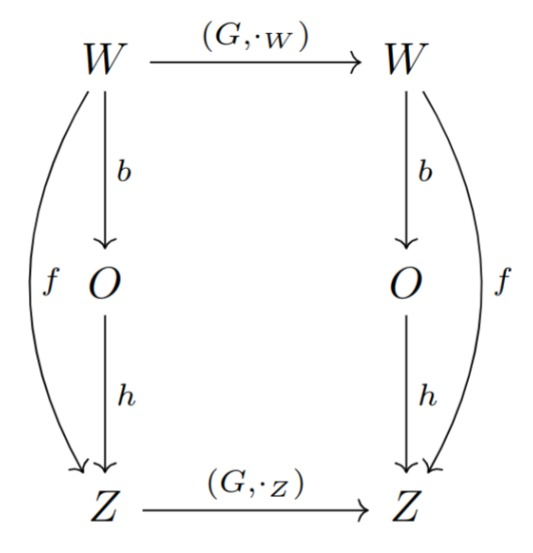
\includegraphics[scale=.3]{group_structure.jpeg}
    \caption{The proposed group structure of the learning problem}
   \end{figure} 
   \end{column} 
  \end{columns}
\end{frame}
\section{Architecture and Loss Propositions}
\begin{frame}{HAE and Two Losses}
  \begin{columns}
    \begin{column}{.6\textwidth}
      \begin{definition}[$N-$step Prediction Loss]
        $\mathcal{L}_{\text{pred}}^N(\rho, h) = \sum_{t}\sum_{j = 1}^{N} || h(o_{t+j}) -  (\prod_{i = 0}^{j-1} \rho(g_{t+i}))h(o_t)||  $
      \end{definition}
      \begin{definition}[$N-$step Reconstruction Loss]
        $\mathcal{L}_{\text{rec}}^N(\rho, h, d) = \sum_{t}\sum_{j = 1}^{N} || o_{t+j} -  d(\prod_{i = 0}^{j-1} \rho(g_{t+i}))h(o_t)||  $
      \end{definition}
   \end{column} 
    \begin{column}{.4\textwidth}
   \begin{figure}
    \centering
    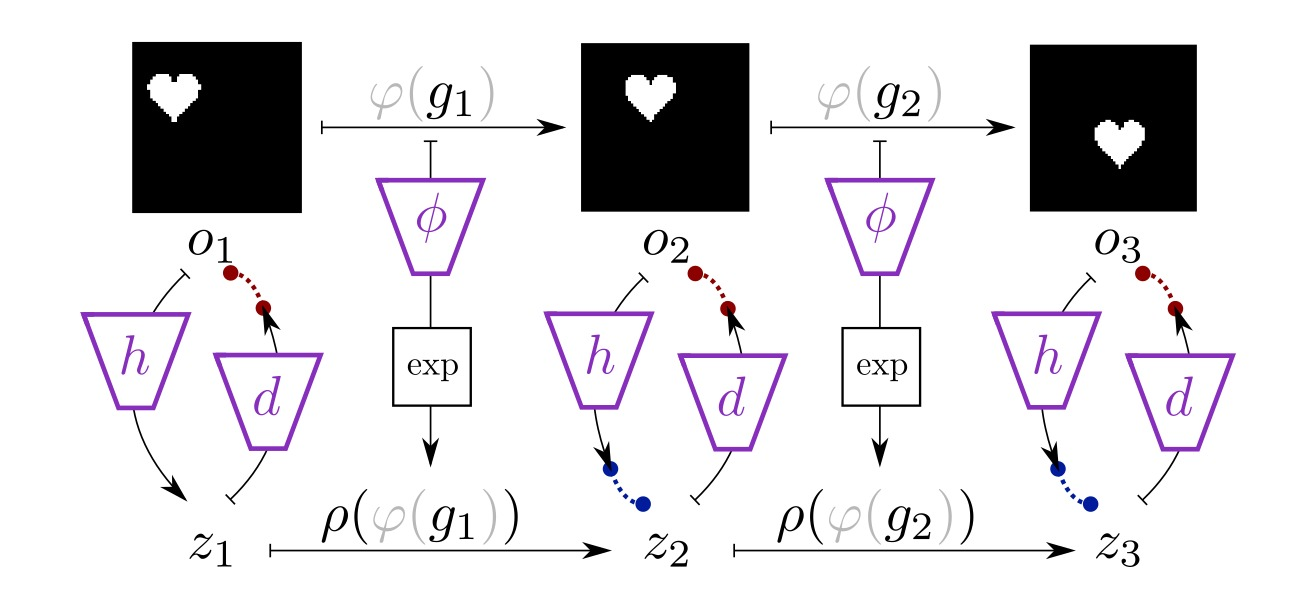
\includegraphics[scale=.1]{hae.jpeg}
    \caption{HAE's Architecture}
   \end{figure} 
   \end{column} 
  \end{columns}
\vspace{10pt}
  A weighted sum of both losses, $\mathcal{L}(\rho, h, d) = \mathcal{L}_{\text{rec}^N}(\rho, h, d) + \gamma \mathcal{L}_{\text{pred}}^N(\rho, h)$, is optimized for.

\end{frame}
\section{Theorem}
\begin{frame}{Restrictions on the Representation Class}
 \begin{theorem}
  If $(\rho, h, d)$ are continuous and minimize the expectation of $\mathcal{L}_{\text{pred}}^2(\rho, h) + \gamma \mathcal{L}_{\text{rec}}^k(\rho, h, d)$, for $k \geq 0$, then $\rho$ is a non-trivial group representation and $(\rho, h)$ is a symmetry-based representation.
 \end{theorem} 
 Informally, a symmetry-based representation is one that satisfies the following: 
 \[ 
 \rho(g_1, g_2, ..., g_n)(z_1 \oplus ... \oplus z_n) = \rho_1(g_1)(z_1)  \oplus ... \oplus \rho_n(g_n)(z_n) \text{~where~} z_i = h(o_i)
 .\]
\end{frame}

\section{Assignment 2}
\begin{frame}{Assignment 2}
  \centering \textbf{The Basics of Group Theory}
  \begin{itemize}
    \item \textbf{Goal}: Understand \textit{just} enough group theory %and differential geometry
      to follow along with the proposition's full statement.
    \item Questions to be addressed:
      \begin{enumerate}
      \item What is a group? What is a subgroup?
      \item What are homomorphisms and isomorphisms?
      \item What is a product group?
      \item What is a group action?
      \item What are diffeomorphisms and homeomorphisms?
      \item What precisely is a manifold? When is it smooth?
      \item What are lie groups and lie algebras?
      \end{enumerate}
      For a more complete treatment of group theory and group actions, refer to \cite{Artin:1998} and \cite{gallier2020differential}.
  \end{itemize}
\end{frame}
\subsection{Preliminary Calculus}
\begin{frame}{Preliminary Calculus}
  \begin{definition}[Convergence of a Series]
    Given a normed vector space $(\mathcal{V}, ||\cdot||)$, a series $\sum_{i = 0}^{\infty} v_i$ is said to converge if the sequence \{$S_n = \sum_{i = 0}^{n} v_i$\} converges to some value $v \in \mathcal{V}$.
  \end{definition}
  \begin{definition}[Cauchy Sequence]
    Given a normed vector space $(\mathcal{V}, ||\cdot||)$, a sequence $\{v_n\}$ is called a Cauchy sequence iff for every $\epsilon > 0$, $\exists N > 0$ such that $\forall m, n > N$, 
      \[ 
      ||v_n - v_m|| < \epsilon
      .\]
      
  \end{definition}
  \begin{definition}[Banach Space]
    A normed vector space is said to be complete, or a \textit{Banach} space, if every Cauchy sequence within the space converges.
  \end{definition}
\end{frame}
\subsection{Groups}
\begin{frame}{Groups}
  A group is a set $G$ equipped with a binary operation $\cdot: G \times G \to G$ such that:
  \begin{itemize}
  \item The law of composition is associative: 
    \[ 
    (a \cdot b) \cdot c = a \cdot (b \cdot c) = a \cdot b \cdot c ~\forall a, b, c \in G
    \]
  \item There exists an identity element $e \in G$ such that:
    \[ 
    e \cdot a = a \cdot e = a ~\forall a \in G
    \]
  \item Every element $a \in G$ has an inverse $a^{-1} \in G$ such that:
    \[ 
    a \cdot a^{-1} = a^{-1} \cdot a = e
    \]
  \end{itemize}
  \textbf{Note:} If the law of composition is commutative, the group is called \textit{abelian}.
\end{frame}
\begin{frame}{Groups}
  \textbf{Examples}
  \begin{itemize}
  \item The set of integers $\mathbb{Z^+}$ under addition is a group.
  \item The set of even integers under addition is a group.
  \item The set of non-zero real numbers $\mathbb{R}^\times$ under multiplication is a group.
  \item The set of odd integers under addition is \textit{not} a group.
  \end{itemize}
\end{frame}
\begin{frame}{Subgroups}
  A subgroup $H$ of a group $G$ is a subset of $G$ that is itself a group under the same law of composition as $G$.

  \textbf{Note:} The identity element of $H$ is the same as that of $G$.
\end{frame}
\begin{frame}{Groups as sets of transformations}
  Groups are often used to formalize and understand sets of transformations. For example:
  \begin{itemize}
  \item $\mathbf{GL}(n, \mathbb{R})$: The \textit{General Linear Group} is the set of all invertible $n \times n$ matrices under matrix multiplication.
  \item $\mathbf{SL}(n, \mathbb{R})$: The \textit{Special Linear Group} is the set of all $n \times n$ matrices with determinant 1 under matrix multiplication.
  \item $\mathbf{O}(n)$: The \textit{Orthogonal Group} is the set of all $n \times n$ orthogonal matrices under matrix multiplication.
  \item $\mathbf{SO}(n)$: The \textit{Special Orthogonal Group} is the set of all $n \times n$ orthogonal matrices with determinant 1 under matrix multiplication.
  \end{itemize}
  \note{Also talk about permutations and how those are groups}
\end{frame}
\begin{frame}{The Cyclic Group}
  If we're given a group $G$, then the cyclic subgroup generated by an element $a \in G$ is the smallest group containing $a$:
  \[ 
    \langle a \rangle = \{a^n | n \in \mathbb{Z}\} = \{... a^{-2}, a^{-1}, 1, a, a^2, ...\}
  .\]
  If, for any $k \in \mathbb{Z}$, $a^k = e$, then the order of $a$ is the smallest such $k$, since after the $k^{th}$ composition, the elements loop back around on themselves.
\end{frame}
\begin{frame}{Homomorphisms}
  \begin{definition}[Homomorphism]
    Let $(G, \cdot)$ and $(H, \circ)$ be groups. A function $\phi: G \to H$ is called a homomorphism if:
    \[
    \phi(a \cdot b) = \phi(a) \circ \phi(b) ~\forall a, b \in G
    \]
  \end{definition}
\end{frame}
\begin{frame}{Examples}
  \begin{itemize}
  \item The determinant function $\text{det}: \mathbf{GL}(n, \mathbb{R}) \to \mathbb{R}^\times$.
  \item The exponential function $\exp: \mathbb{R}^+ \to \mathbb{R}^\times$.
  \item The absolute value function $|\cdot|: \mathbb{C}^\times \to \mathbb{R}^\times$.
  \end{itemize}
  \begin{definition}[The Trivial Homomorphism]
    The homomorphism $\varphi: G \to G'$ such that $\varphi(g) = e_{G'}$ for all $g \in G$ is called the trivial homomorphism.
  \end{definition}
\end{frame}
\begin{frame}{The Image and the Kernel}
  Let $\varphi: G \to G'$  be a homomorphism. 
  \begin{definition}[The Image of a Homomorphism]
  The image of $\varphi$, denoted $\text{im}(\varphi)$, is the set of all elements in $G'$ that are the image of some element in $G$ under $\varphi$:
  \[ 
    \text{im}\varphi = \{x \in G' | x = \varphi(a) ~\text{for some } a \text{ in } G\}
  .\]
  \end{definition} 
  \begin{definition}[The Kernel of a Homomorphism]
    The kernel of $\varphi$, denoted by $\text{ker}(\varphi)$, is the set of all elements in $G$ that are mapped to the identity element of $G'$:
    \[ 
    \text{ker}\varphi = \{a \in G | \varphi(a) = e_{G'}\}
    .\]
    
  \end{definition}
\end{frame}
\begin{frame}{Isomorphisms}
  An isomorphism is a bijective homomorphism.
  \begin{definition}[Isomorphic Groups]
    Two groups $G$ and $G'$ are said to be isomorphic if there exists an isomorphism $\varphi: G \to G'$. This is denoted by $G \cong G'$ or by $G \approx G'$.
    \end{definition}
    \begin{lemma}
      If $\varphi: G \to G'$ is an isomorphism, then $\varphi^{-1}: G' \to G$ exists, and is also an isomorphism.
    \end{lemma}
\end{frame}
\begin{frame}{Product Groups}
  If we have two groups $G$ and $G'$, then the product group is the set $G \times G'$, with each group's law of composition applied component-wise:
  \begin{gather}
    (a, a'), (b, b') \in G \times G' \\
    \implies (a, a') \cdot (b, b') = (a \cdot b, a' \cdot b')
  \end{gather}
  \textbf{Note:} A isomorphism from a group to itself is called an automorphism.
\end{frame}
\begin{frame}{Product Groups}
  \begin{columns}
    \begin{column}{.65\textwidth}
      The product group can be understood in terms of its factors through the following four homomorphisms:
      \begin{itemize}
      \item $i(x) = (x, 1), i'(x') = (1, x')$
      \item $p(x, x') = x, p'(x, x') = x'$
      \end{itemize}
    The injective homomorphisms $i$ and $i'$ map the groups $G$ and $G'$ to their images, $G \times 1$ and $1 \times G'$ respectively.
    The surjective homomorphisms $p$ and $p'$ map their kernels, $1 \times G'$ and $G \times 1$ respectively, to the identity elements of $G$ and $G'$.
    \end{column}
    \begin{column}{.33\textwidth}
     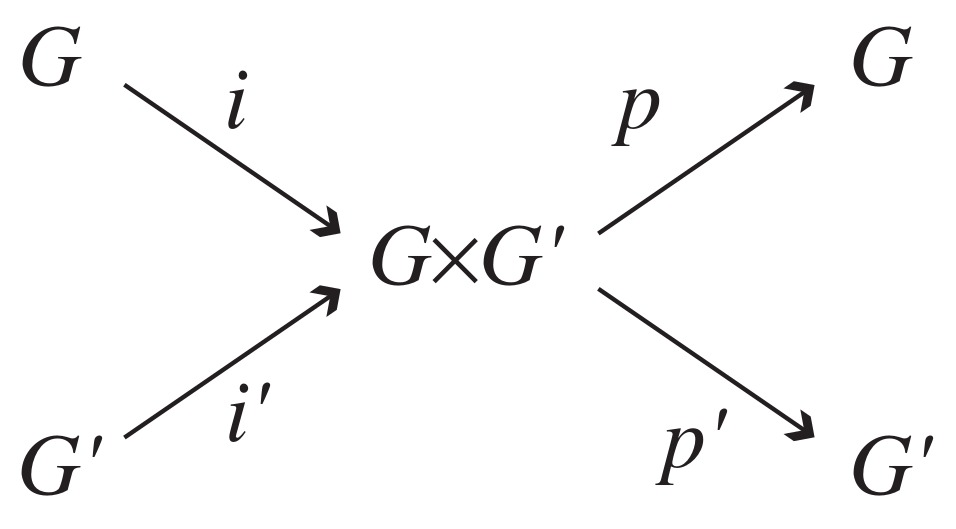
\includegraphics[width=\linewidth]{group_product.jpeg} 
    \end{column}
      
  \end{columns}
\end{frame}
\begin{frame}{Example}
  The group $\mathcal{T}_3$ consisting of translations of an object in 3D space can be thought of as the group product of the translation groups $\mathcal{X}, \mathcal{Y}, ~\text{and} ~\mathcal{Z}$ along the $X, Y ~\text{and}~ Z$ axes, i.e.
  \[ 
  \mathcal{T}_3 \cong \mathcal{X} \times \mathcal{Y} \times \mathcal{Z}
  .\]
  
\end{frame}
\begin{frame}{Group Action}
  \begin{definition}[Group Action]
   Given a set $X$  and a group $G$, an action of $G$ on $X$ is a function $\varphi: G \times X \to X$, such that:
   \begin{align}
     \varphi(g, \varphi(h, x)) = \varphi(gh, x) &~\forall g, h \in G, x \in X \\
     \varphi(e, x) = x &~\forall x \in X
   \end{align}
  \end{definition}
  Normally, we write $\varphi(g, x)$ as $g \cdot x$ or $gx$, making the above rules
  \begin{align}
    g \cdot (h \cdot x) = (gh) \cdot x &~\forall g, h \in G, x \in X \\
    e \cdot x = x &~\forall x \in X
  \end{align}
  \textbf{Note:} If the set $X$ is such that the group action $\varphi: G \times X \to X$ exists, then $X$ is called a $G-$set.
\end{frame}
\begin{frame}{Group Action}
  While $\varphi$ is a function that ranges across $g \in G$ and $x \in X$, we can construct a new function for each $g \in G$, where $g$ is treated as a parameter: \[ 
    \varphi_g: X \to X, \varphi_g(x) = gx
  .\]

  Note that $\varphi_g$ has an inverse, namely $\varphi_{g^{-1}}$. This means that $\varphi_g$ is a bijection from $X$ to $X$, making it a permutation of $X$.

  If we define, by $\mathcal{G}_X$, the group of permutations of $X$, then the map $g \mapsto \varphi_g$ is a homomorphism from $G$ to $\mathcal{G}_X$.
\end{frame}
\begin{frame}{Equivariant Maps}
  \begin{definition}[Equivariant Map]
    Given two $G-$sets $X$ and $Y$, a map $f: X \to Y$ is called equivariant iff $\forall x \in X$ and $\forall g \in G$, 
    \[ 
    f(g \cdot x) = g \cdot f(x)
    .\]
  \end{definition}
  \centering 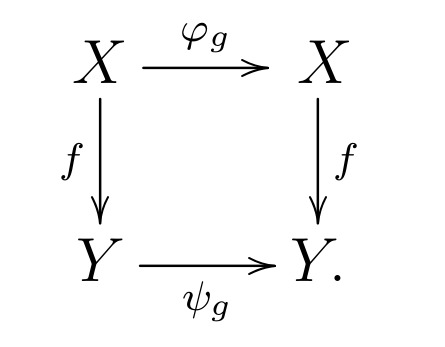
\includegraphics[width=.5\linewidth]{equivariant_map.jpeg}
  \note{Talk about contrasting notions of compositionality, and how equivariance is more general condition than homomorphicity}
\end{frame}
\begin{frame}{References}
  \bibliographystyle{amsalpha}
  \bibliography{references}

  
\end{frame}
\end{document}
